
\begin{figure*}[htpb]
  \centering
   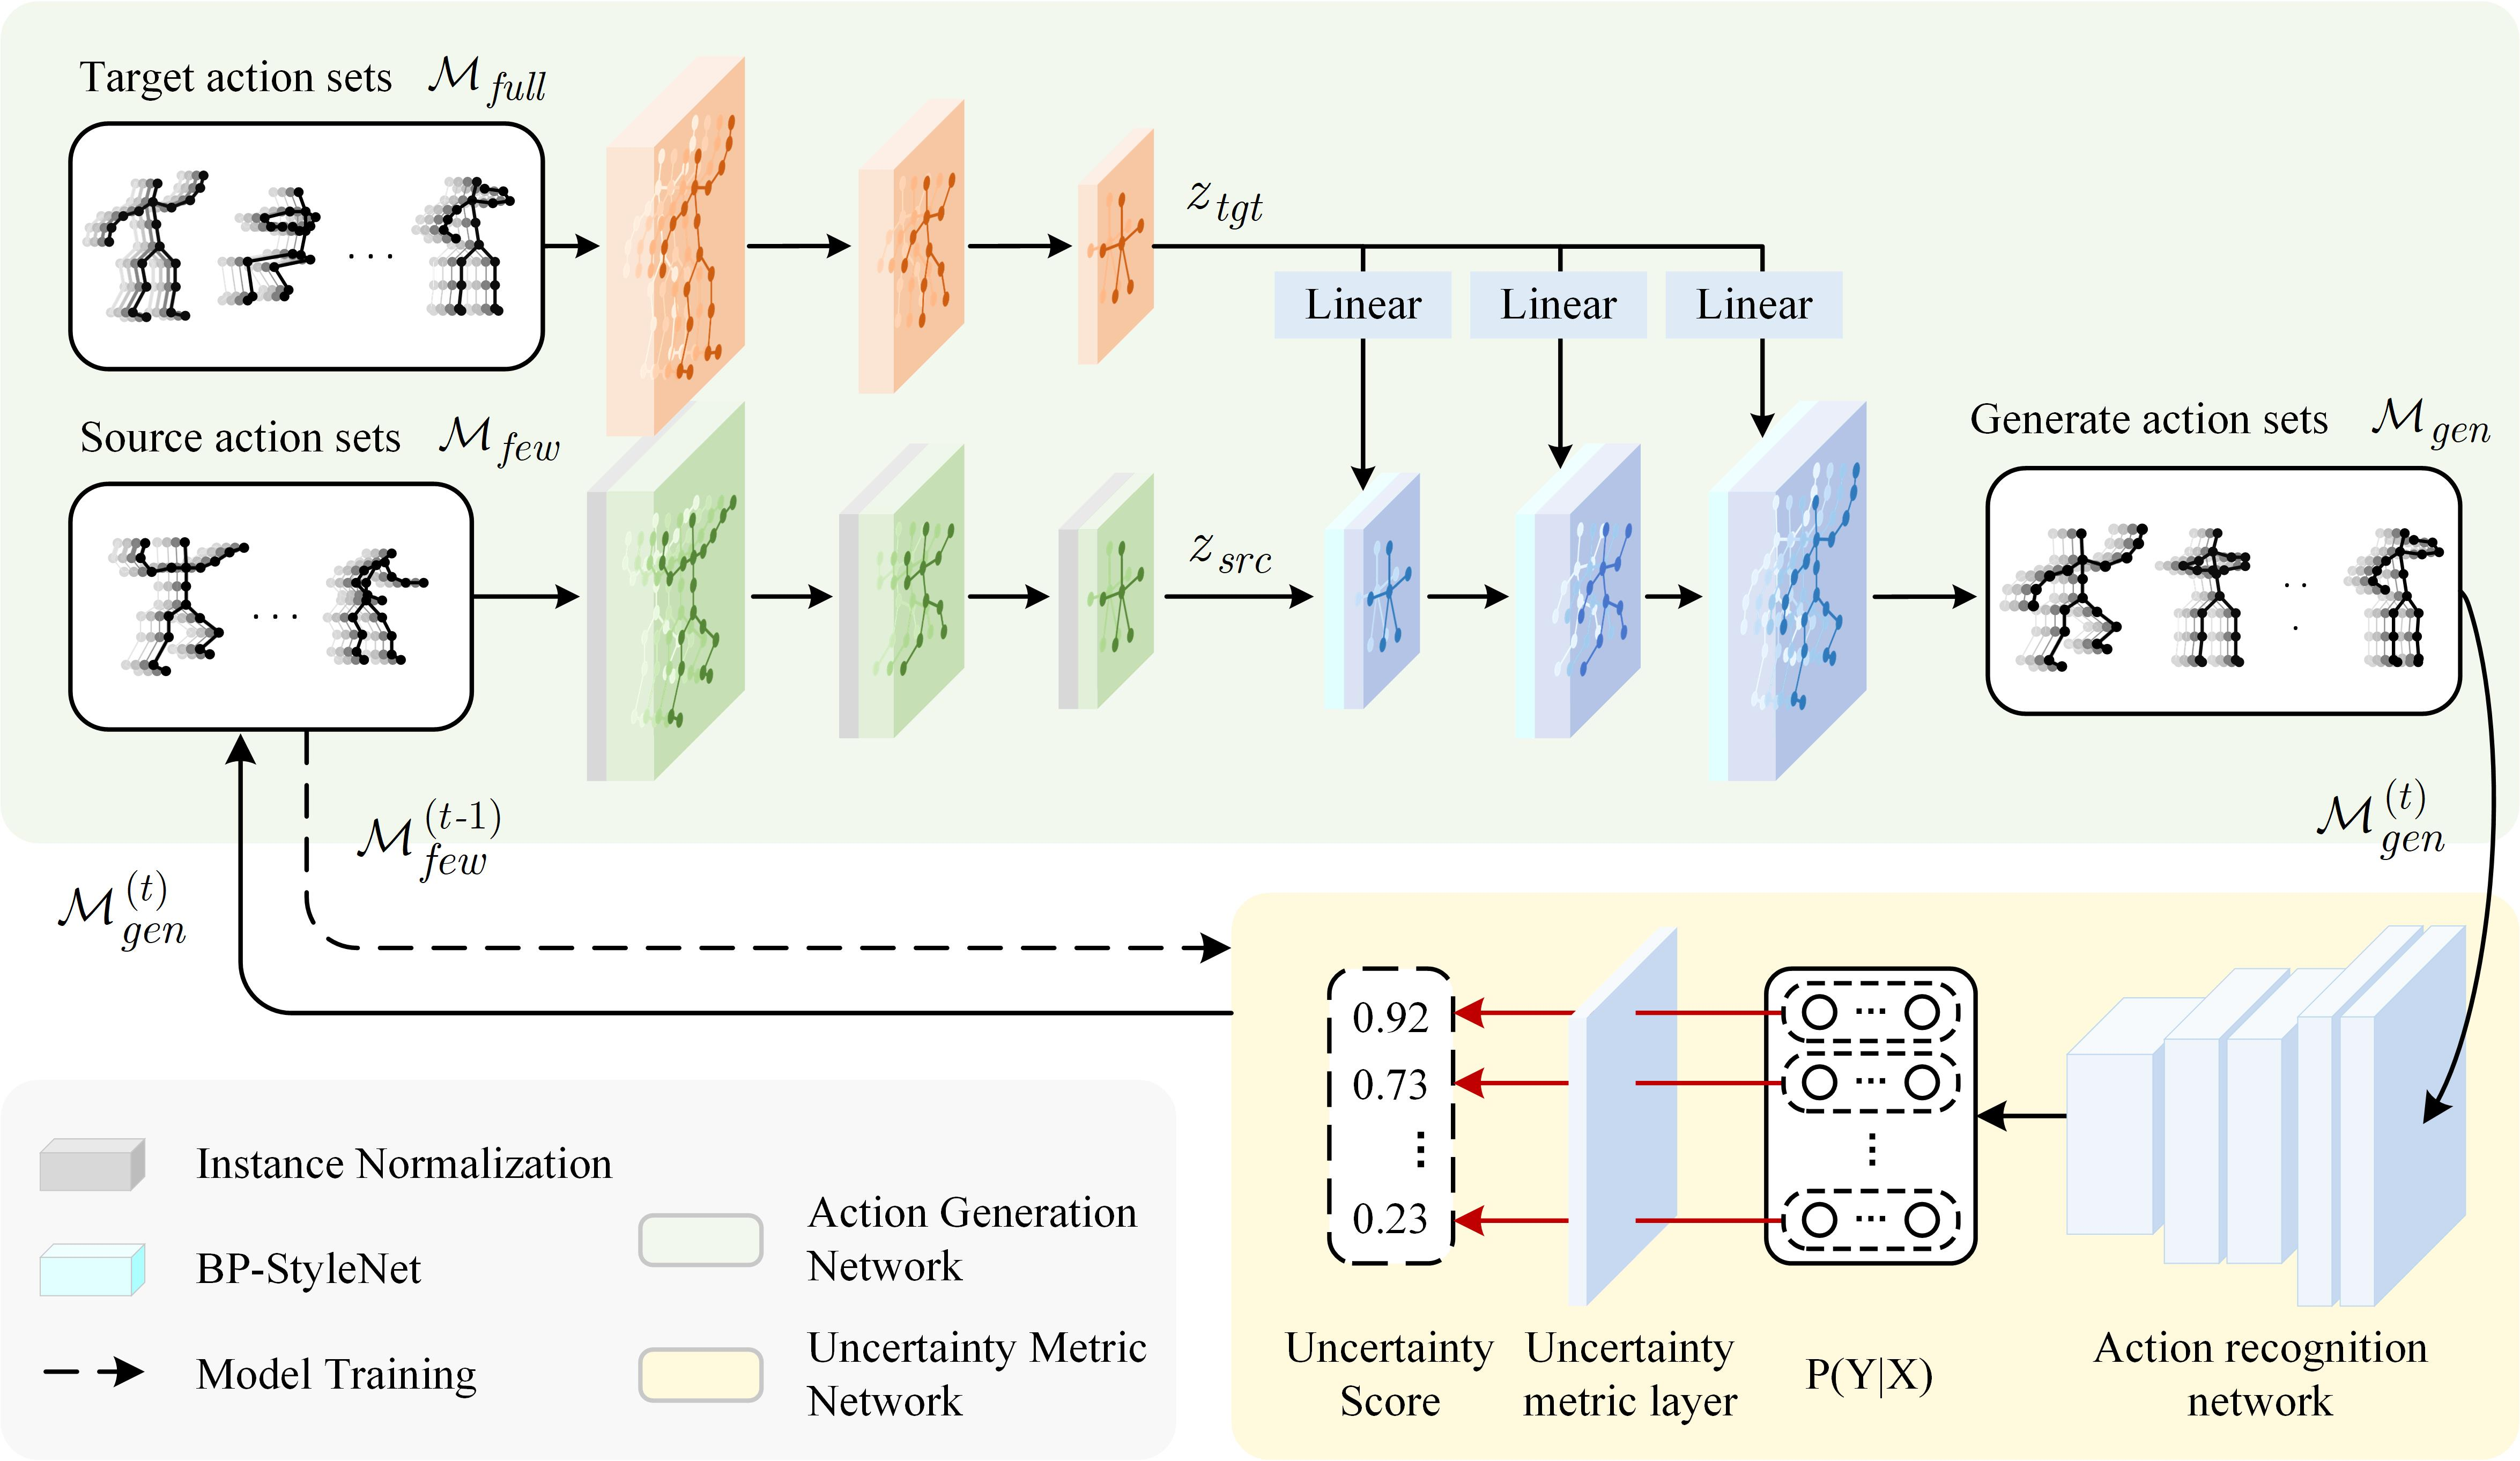
\includegraphics[width=0.8\linewidth]{figures/Fig1.jpg}

   \caption{The overall network architecture of our AGN framework. }
   \label{fig:1}
\end{figure*}

\section{Method}

\subsection{Overview}

Figure \ref{fig:1} shows the overall architecture of the AGN framework, consisting of MGN and UMN. 
The MGN generates new actions, and the UMN evaluates the generated actions and inversely guides the generation of MGN. 
We construct a human action set $\mathcal{M}=\mathcal{M}_{train}\cup \mathcal{M}_{unseen}$ using 3D skeletal data from NTU-RGB+D 60  \cite{shahroudy2016ntu}, where $\mathcal{M}_{train}\cap \mathcal{M}_{unseen}=\varnothing$. 
In addition, we define different action subsets. 
The AGN's input is a complete target action set $\mathcal{M}_{full}$ and a one-shot or few-shot source action set $\mathcal{M}_{few}$. The final output is a complete action set $\mathcal{M}_{gen}$ of equal size $\mathcal{M}_{full}$. The action is denoted as $\textbf{M}_{src}\in\mathcal{M}_{few}, \textbf{M}_{tgt}\in\mathcal{M}_{full}$, and $\textbf{M}_{gen}\in\mathcal{M}_{gen}$. 

The MGN uses spatio-temporal graph convolutional layers as the basis to construct the encoder and decoder, connecting the high and low dimensional feature layers of the human skeletal graph structure by graph upsampling and downsampling \cite{yan2019convolutional, jang2022motion}.
The encoder extracts features for the skeletal morphology and the category information of the action, respectively. The decoder outputs the new action by fusing the multi-scale spatio-temporal features of the source and target actions via the BP-StyleNet Layer \cite{jang2022motion}.
The UMN guides the MGN to generate high-quality action. 
Specifically, the UMN obtains the a posteriori probability of each action via a recognition network. Then, the uncertainty score is obtained via an uncertainty metrics layer to provide a basis for sample selection.

\subsection{Action Generation Network}

\textbf{Graph Upsampling and Downsampling. }
A practical method for extracting features in image generation is progressive upsampling and downsampling. The upsampling gradually improves the image resolution and increases the local details, and the downsampling can aggregate the image features and reduce the noise. 
The upsampling and downsampling are generally implemented through Unpooling and Pooling. It proved effective in graph convolutional neural networks for skeletal data\cite{jang2022motion, yan2019convolutional, ParkSoomin2021Diverse}. 
Following this idea, we incorporate the upsampling and downsampling methods combined with information entropy into the spatial-temporal graph to extract local and global features. 

\textbf{Action Encoder. }
We developed the action encoder similar to VGG16 \cite{simonyan2014very} to map human actions to latent space using graph upsampling and spatio-temporal graph convolutional layers. Given an action $\textbf{M}_s$, the encoding process is written as: 

\begin{equation}\label{e2}
z_s=E_s(\textbf{M}_s),
\end{equation}

\noindent where $s\in \{src, tgt\}$.
The action encoder consists of a source encoder and a target encoder. 
Each encoder $E_s$ is a concatenation of multi-level encoding blocks $E_s^i$ to gradually extract the latent feature $z_s^i=E_s^i(z_s^{i-1})$, where $i\in \{1,2,3\}$, and $z_s^i$ is the action feature obtained after each encoding block. 

The source encoding block $E^i_{src}$ consists of instance normalization layer (IN), ST-GCN, and graph downsampling (GD) to extract source action features gradually. 
In the target encoder, we wish to preserve the morphological features of the action to combine with the category features of the source action to form a unique new action. Therefore, it consists only of ST-GCN and GD. 

\textbf{Feature Decoder. }
The feature decoder fuses the category features $z_{src}$ of the source action with the morphological features $z_{tgt}$ of the target action to synthesise a new action $\textbf{M}_{gen}$. The dncoding process is written as: 

\begin{equation}\label{e5}
\textbf{M}_{gen}=D(z_{src}, z_{tgt}).
\end{equation}

\noindent The decoder is similar in structure to the encoder and consists of three decoding blocks and three linear layers. 
The three decoding blocks recover the action sequences step-by-step by fusing $z_{tgt}$ and $\hat{z}^0_{dec}(=z_{src})$, defined as:

\begin{equation}\label{e6}
\hat{z}^i_{dec}=D^i(\hat{z}^{i-1}_{dec}, L^i(z_{tgt})),
\end{equation}

\noindent where $i\in \{1,2,3\}$, $\hat{z}_{dec}^i$ is the action feature output from each decoding block, and $L^i$ is the linear layer mapping the deep feature $z_{tgt}$ to the same feature map size as the output of each decoding blocks.

We use Body Part Adaptive Instance Normalisation (BP-AdaIN) and Body Part Attention Network (BP-ATN) in the decoding block from Motion Puzzle \cite{jang2022motion}, where BP-AdaIN applies AdaIN \cite{gatys2016image, saito2020coco} according to the body parts, extending the network's degree of freedom, and more flexible fusion of the features of each part of the target and the source action. 
The BP-ATN constructs the feature attention mapping of the target and source actions. 
BP-AdaIN and BP work together to extract local and global features of the target action.

\subsection{Uncertainty Metric Network}

\textbf{Action Recognition Network}. 
The prediction vectors are obtained from the action recognition model, thereby calculating the uncertainty score. 
Our task is oriented towards data generation for action recognition, and thus, ST-GCN is adopted as the task model. 
At the first iteration, $\mathcal{M}^{(1)}_{gen}=MGN(\mathcal{M}^{(0)}_{few},\mathcal{M}_{full})$ is obtained by inputting $\mathcal{M}^{(0)}_{few}$ into the MGN. 
Meanwhile, the task model is trained using $\mathcal{M}^{(0)}_{few}$. Finally, prediction vectors are generated for each action. 
Starting from the second iteration, $\mathcal{M}^{(t)}_{few}=\mathcal{M}^{(t-1)}_{few}\cup\mathcal{M}^{(t)}_{gen}, t\in[1,iter]$. 
Given that the number of categories is $L$, then $Y = p(\mathcal{M}^{(t)}_{gen}|\mathcal{M}^{(t-1)}_{few})\in\mathbb{R}^{K\times L}$,  where $K$ is the number of generating samples, and $p(A|B)$ denotes the prediction vectors produced by the action recognition model trained under dataset $B$ for dataset $A$.

\textbf{Uncertainty Metrics}. 
The uncertainty score of the prediction vector is calculated by the uncertainty metric. The uncertainty score is calculated as follows:

\begin{equation}\label{e7}
S(Y)=I-\frac{Var(Y'[k])}{Var(Y[k])}\times max(Y[k]),
\end{equation}

\noindent where $I$ is a full one-vector of length $K$, then $S(Y)\in\mathbb{R}^K, k\in [1,K]$. The $Var(Y[k])$ can be formulated as:

\begin{equation}\label{e8}
Var(Y[k])=\frac{1}{L}\sum_l (Y[l,k]-\frac{1}{L})^2.
\end{equation}

\noindent The $Var(Y'[k])$ is the minimum variance of the same vector as the maximum value of $Y[k]$, denoted as:

\begin{equation}\label{e9}
\begin{aligned}
&Var(Y’[k])=\\
&\frac{1}{L}((max(Y[k])-\frac{1}{L})^2+(L-1)(\frac{1-max(Y[k])}{L-1}-\frac{1}{L})^2).
\end{aligned}
\end{equation}

\noindent The maximum value in $Y'[k]$ is the same as the maximum value of $Y[k]$, and the other elements are $\frac{1-max(Y[k])}{L-1}$. 
Therefore, $\frac{Var(Y'[k])}{Var(Y[k])}$ represents the degree of concentration of the probability distribution of the predicted vectors. It ensures that each score ranges from 0 to 1 and is negatively correlated with the maximum vector, i.e., a smaller $max(Y[k])$ indicates greater uncertainty.
Finally, the action data is selected based on this score to form the action set $\mathcal{M}_{gen}$.

\subsection{Training}

We train the action generation network end-to-end, given the source action $\textbf{M}_{src}\in\mathcal{M}_{src}$ and the target action set $\textbf{M}_{tgt}\in\mathcal{M}_{tgt}$, and optimize the network with the following loss function. 

\textbf{Reconstruction loss} and \textbf{Cycle consistency loss} are outstanding in motion style transfer \cite{jang2022motion, aberman2020unpaired, ParkSoomin2021Diverse, 2016A}.
Reconstruction loss gives the network the ability to reconstruct a movement. For each action in the action set, the network can reconstruct the action after feature disentanglement and feature fusion. The new action should have both source action category features and target action morphological features. Therefore, the encoders $E_{src}$ and $E_{tgt}$ are used to disentangle the features of $\textbf{M}_{gen}$ and the acquired features are used to compute the cycle consistency loss with the features of the source and target actions, respectively. 

\textbf{Feature triplet loss. }
In order to make the category features of the action more apparent in the latent space, a triplet loss is used during training to make the same category of actions clustered with each other and different categories of actions far away from each other so that the network captures the similarities and differences between action features. 

\begin{equation}\label{e12}
\begin{aligned}
&\mathcal{L}_{trip}=\\
&\mathbb{E}_{\textbf{M}^t_i,\textbf{M}^t_j,\textbf{M}^s_k\sim\mathcal{M}}(||E_{src}(\textbf{M}^t_i)-E_{src}(\textbf{M}^t_j)||-\\
&||E_{src}(\textbf{M}^t_i)-E_{src}(\textbf{M}^s_k)||+\delta),
\end{aligned}
\end{equation}

\noindent where $\textbf{M}^t_i$ and $\textbf{M}^t_j$ represent two motions of the same category,  $\textbf{M}^t_{i,j}$ and $\textbf{M}^s_k$ denote two motions of the different category, so $t\neq s, i\neq j\neq k$. The boundary value $\delta=5$. 

The total objective function of the MGN is thus: 

\begin{equation}\label{e13}
\mathcal{L}_{total}=\lambda_{rec}\mathcal{L}_{rec}+\lambda_{cyc}\mathcal{L}_{cyc}+\lambda_{trip}\mathcal{L}_{trip},
\end{equation}

\noindent where $\lambda_{rec}, \lambda_{cyc},$ and $\lambda_{trip}$ are the hyperparameters of each loss term. 1, 0.5, and 0.5, respectively, in our experiments.